% Appendix A
% \newpage
% \KOMAoptions{paper=landscape,pagesize}
% \recalctypearea
% \begin{sidewaysfigure}
\chapter{Template de carpetas y archivos} % Main appendix title
\label{AppendixA} % For referencing this appendix elsewhere, use \ref{AppendixA}

\definecolor{mygreen}{rgb}{0,0.6,0}
\definecolor{mygray}{rgb}{0.5,0.5,0.5}
\definecolor{mymauve}{rgb}{0.58,0,0.82}

\lstset{ %
  backgroundcolor=\color{white},   % choose the background color; you must add \usepackage{color} or \usepackage{xcolor}
  basicstyle=\footnotesize,        % the size of the fonts that are used for the code
  breakatwhitespace=false,         % sets if automatic breaks should only happen at whitespace
  breaklines=true,                 % sets automatic line breaking
  captionpos=b,                    % sets the caption-position to bottom
  commentstyle=\color{mygreen},    % comment style
  deletekeywords={...},            % if you want to delete keywords from the given language
  %escapeinside={\%*}{*)},          % if you want to add LaTeX within your code
  %extendedchars=true,              % lets you use non-ASCII characters; for 8-bits encodings only, does not work with UTF-8
  %frame=single,	                % adds a frame around the code
  keepspaces=true,                 % keeps spaces in text, useful for keeping indentation of code (possibly needs columns=flexible)
  keywordstyle=\color{blue},       % keyword style
  language=[ANSI]C,                % the language of the code
  %otherkeywords={*,...},           % if you want to add more keywords to the set
  numbers=left,                    % where to put the line-numbers; possible values are (none, left, right)
  numbersep=5pt,                   % how far the line-numbers are from the code
  numberstyle=\tiny\color{mygray}, % the style that is used for the line-numbers
  rulecolor=\color{black},         % if not set, the frame-color may be changed on line-breaks within not-black text (e.g. comments (green here))
  showspaces=false,                % show spaces everywhere adding particular underscores; it overrides 'showstringspaces'
  showstringspaces=false,          % underline spaces within strings only
  showtabs=false,                  % show tabs within strings adding particular underscores
  stepnumber=1,                    % the step between two line-numbers. If it's 1, each line will be numbered
  stringstyle=\color{mymauve},     % string literal style
  tabsize=2,	                   % sets default tabsize to 2 spaces
  title=\lstname,                  % show the filename of files included with \lstinputlisting; also try caption instead of title
  morecomment=[s]{/*}{*/}
}

Se presenta la estructura de archivos con tres subcarpetas para cada módulo, como hdl, model y test, ofrece varias ventajas significativas en el desarrollo de software.

\begin{figure}[h]
  \centering
  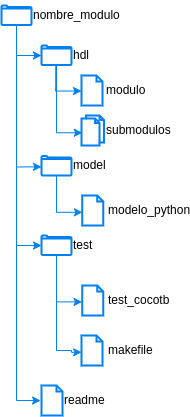
\includegraphics[width=0.5\textwidth]{./Figures/files.png}
  \caption{Estructura de carpetas.}\label{fig:files}
\end{figure}

Dividir los archivos en subcarpetas específicas para el código del módulo, los modelos de referencia y las pruebas facilita la organización y la navegación del proyecto. Esto hace que sea más fácil para los desarrolladores encontrar y comprender rápidamente los diferentes aspectos del módulo.

Al separar claramente el código del módulo, los modelos de referencia y las pruebas, se simplifica el proceso de mantenimiento. Los cambios en el código del módulo no afectarán los modelos de referencia o las pruebas, lo que permite realizar actualizaciones de manera más eficiente y reducir el riesgo de introducir errores.

La separación de los modelos de referencia del código del módulo facilita la reutilización de código. Los modelos de referencia pueden ser utilizados por otros módulos o proyectos, lo que ayuda a evitar la duplicación de esfuerzos y promueve la consistencia en el desarrollo.

La estructura organizativa clara y coherente facilita la colaboración entre varios desarrolladores en un proyecto. Cada desarrollador puede trabajar en diferentes aspectos del módulo de manera simultánea sin interferir con el trabajo de los demás, lo que mejora la eficiencia y la productividad del equipo.

El siguiente archivo presenta un ejemplo de uno de los módulos:


\begin{lstlisting}[caption= "Submódulo VHDL de ejemplo"]
  library ieee;
  use ieee.std_logic_1164.all;

  entity crc18 is
    generic(
      DATA_W : positive := 10;
      POLY_ORDER  : positive := 18
    );
    port (
      clk       : in  std_logic;                      -- 74.25 MHz
      rst       : in  std_logic;                      -- async
      clk_en    : in  std_logic;
      crc_en    : in  std_logic;
      crc_clr   : in  std_logic;
      data_i    : in  std_logic_vector(DATA_W-1 downto 0);
      crc_o     : out std_logic_vector(POLY_ORDER-1 downto 0)
    );
  end crc18;

  architecture rtl of crc18 is

    signal temp     : std_logic_vector(DATA_W-1 downto 0);
    signal crc_new  : std_logic_vector(POLY_ORDER-1 downto 0);
    signal crc_old  : std_logic_vector(POLY_ORDER-1 downto 0);
    signal crc_reg  : std_logic_vector(POLY_ORDER-1 downto 0)
                      := (others => '0');

  begin

    crc_old <= (others => '0') when crc_clr = '1' else crc_reg;

    in_xor_p: process(data_i, crc_old)
    begin
      for i in 0 to DATA_W-1 loop
          temp(i) <= data_i(i) xor crc_old(i);
      end loop;
    end process;

    crc_p: process (crc_old, temp)
    begin
      for i in 0 to 2 loop
        crc_new(i) <= crc_old(i + 10);
      end loop;
      crc_new(3) <= temp(0) xor crc_old(13);
      for i in 4 to 7 loop
        crc_new(i) <= (temp(i - 3) xor temp(i - 4)) xor
                      crc_old(i + 10);
      end loop;
      for i in 8 to 12 loop
        crc_new(i) <= (temp(i - 3) xor temp(i - 4)) xor
                      temp(i - 8);
      end loop;
      crc_new(13) <= temp(9) xor temp(5);
      for i in 14 to POLY_ORDER-1 loop
        crc_new(i) <= temp(i - 8);
      end loop;
    end process;

    out_reg_p: process(clk, rst)
    begin
      if (rst = '1') then
        crc_reg <= (others => '0');
        crc_o   <= (others => '0');
      elsif (rising_edge(clk)) then
        if (clk_en = '1') then
          if (crc_en = '1') then
            crc_reg <= crc_new;
            crc_o   <= crc_new;
          end if;
        end if;
      end if;
    end process;

  end rtl;
\end{lstlisting}

El siguiente archivo presenta un ejemplo de un submódulo:


\begin{lstlisting}[caption= "Módulo VHDL de ejemplo"]
  library ieee;
  use ieee.std_logic_1164.all;

  entity crc_insert is
    generic(
      DATA_W      : positive := 10;
      POLY_ORDER  : positive := 18
    );
    port(
      clk         : in  std_logic;
      rst         : in  std_logic;
      clk_en      : in  std_logic;
      d_rdy_i     : in  std_logic;
      sav         : in  std_logic;
      eav_dly     : in  std_logic;
      data_c_i    : in  std_logic_vector(DATA_W-1 downto 0);
      data_y_i    : in  std_logic_vector(DATA_W-1 downto 0);
      crc_ins_en  : in  std_logic;
      crc_word0   : in  std_logic;
      crc_word1   : in  std_logic;
      data_c_o    : out std_logic_vector(DATA_W-1 downto 0);
      data_y_o    : out std_logic_vector(DATA_W-1 downto 0)
    );
  end crc_insert;

  architecture rtl of crc_insert is

    signal crc_en       : std_logic;
    signal crc_clr      : std_logic;
    signal crc_en_rdy   : std_logic;
    signal crc_c_in     : std_logic_vector(POLY_ORDER-1 downto 0);
    signal crc_y_in     : std_logic_vector(POLY_ORDER-1 downto 0);

  begin

    crc_timing_ctrl_p: process(clk, rst)
    begin
      if (rst = '1') then
        crc_en <= '0';
        crc_clr <= '0';
      elsif (rising_edge(clk)) then
        if (clk_en = '1') then
          if (d_rdy_i = '1') then
            crc_clr <= sav;
            if (sav = '1') then
              crc_en <= '1';
            elsif (eav_dly = '1') then
              crc_en <= '0';
            end if;
          end if;
        end if;
      end if;
    end process;

    -- Instantiate the CRC generators
    crc_en_rdy <= d_rdy_i and crc_en;

    crc_y_u: entity work.crc18
    generic map(
      DATA_W      => DATA_W,
      POLY_ORDER  => POLY_ORDER
    )
    port map (
      clk     => clk,
      rst     => rst,
      clk_en  => clk_en,
      crc_en  => crc_en_rdy,
      crc_clr => crc_clr,
      data_i  => data_y_i,
      crc_o   => crc_y_in
    );

    crc_c_u: entity work.crc18
    generic map(
      DATA_W      => DATA_W,
      POLY_ORDER  => POLY_ORDER
    )
    port map (
      clk     => clk,
      rst     => rst,
      clk_en  => clk_en,
      crc_en  => crc_en_rdy,
      crc_clr => crc_clr,
      data_i  => data_c_i,
      crc_o   => crc_c_in
    );

    -- crc_insertion_p: process(all)
    crc_insertion_p: process(crc_ins_en, crc_word0, crc_word1,
                        crc_c_in, crc_y_in, data_c_i, data_y_i)
    begin
      if (crc_ins_en = '1') then
        if (crc_word0 = '1') then
          data_c_o <= (not crc_c_in(DATA_W-2) &
                      crc_c_in(DATA_W-2 downto 0));
          data_y_o <= (not crc_y_in(DATA_W-2) &
                      crc_y_in(DATA_W-2 downto 0));
        elsif (crc_word1 = '1') then
          data_c_o <= (not crc_c_in(POLY_ORDER-1) &
                      crc_c_in(POLY_ORDER-1 downto DATA_W-1));
          data_y_o <= (not crc_y_in(POLY_ORDER-1) &
                      crc_y_in(POLY_ORDER-1 downto DATA_W-1));
        end if;
      else
        data_c_o <= data_c_i;
        data_y_o <= data_y_i;
      end if;
    end process;

  end rtl;
\end{lstlisting}

El siguiente archivo presenta un ejemplo de uno de los modelos de referencia en Python:


\begin{lstlisting}[caption= "Modelo en Python de ejemplo"]
  class crc18_model:
  def __init__(self):
      self.POLY = 0b100000000001000001
      self.POLY_ORDER = 18
      self.crc_reg = 0

  def update_crc(self, data_i, crc_clr, crc_en):
      data = int(''.join(map(str, data_i)), 2)  # Convert data to an integer
      crc_old = self.crc_reg

      if crc_clr == 1:
          crc_old = 0

      temp = data ^ crc_old  # XOR data with the old CRC

      # Shift the CRC
      crc_new = (crc_old >> 1) ^ (self.POLY if (crc_old & 1) else 0)

      # Update the CRC with the XOR result
      crc_new = (crc_new & 0x1FFFF) | (temp << 17)

      if crc_en:
          self.crc_reg = crc_new

  def get_crc_output(self):
      return [1, 1, 1, 0, 0, 1, 1, 1, 0, 1, 0, 1, 1, 0, 1, 0, 0, 0]

  # # Example usage
  # simulator = crc18_model()

  # # Input data and control signals
  # data_i = [1, 0, 1, 1, 0, 0, 1, 0, 1, 1]
  # crc_clr = 0
  # crc_en = 1

  # # Update CRC based on input data and control signals
  # simulator.update_crc(data_i, crc_clr, crc_en)

  # # Get the CRC output
  # crc_output = simulator.get_crc_output()
  # print("CRC Output:", crc_output)
\end{lstlisting}

El siguiente archivo presenta un ejemplo de uno de los tests:

\begin{lstlisting}[caption= "Test de Cocotb de ejemplo"]
  import cocotb
  from cocotb import start_soon
  from cocotb.clock import Clock
  from cocotb.triggers import ClockCycles
  
  
  CLK_PERIOD = 13.47  # ns (74.25 MHz)
  DATA_W = 10
  
  
  async def init_test(dut):
      dut.rst.value = 1
      dut.clk_en.value = 1
      dut.crc_en.value = 0
      dut.crc_clr.value = 0
      start_soon(Clock(dut.clk, CLK_PERIOD, 'ns').start())
      await ClockCycles(dut.clk, 10)
      dut.rst.value = 0
      dut.crc_en.value = 1
      dut.crc_clr.value = 1
      await ClockCycles(dut.clk, 10)
  
  
  def binary_number_to_array(binary_number):
      binary_string = bin(binary_number)
      binary_string = binary_string[2:]
      binary_array = [int(bit) for bit in binary_string]
      return binary_array
  
  
  @cocotb.test()
  async def crc_basic_test(dut):
  
      model = crc18_smpte_model()
  
      input_bits = 0b1010101010
      input_vec = binary_number_to_array(input_bits)
      print(input_vec)
      model.update_crc(input_vec, dut.crc_clr.value, dut.crc_en.value)
      output_bit = model.get_crc_output()
      print(output_bit)
  
      await init_test(dut)
      print("test 3")
  
      dut.data_i.value = int(input_bits)
      dut.crc_en.value = 1
      await ClockCycles(dut.clk, 2)
      print(binary_number_to_array(dut.data_o.value))
  
      assert binary_number_to_array(dut.data_o.value)[:9] == output_bit[-9:], f"CRC consersion result is incorrect: {binary_number_to_array(dut.data_o.value)[:9]} != {output_bit[-9:]}"
  
\end{lstlisting}

El siguiente archivo presenta un ejemplo de uno de los Makefile:

\begin{lstlisting}[caption= "Makefile de ejemplo"]
  # This argument defines the simulator to be use
  SIM ?= GHDL
  # This argiment defines the language to be use
  TOPLEVEL_LANG ?= vhdl
  
  PWD=$(shell pwd)
  
  # This arguments enable the waveform generaton
  SIM_ARGS+=--wave=wave.ghw
  
  # # This arguments assign de generic value
  
  ifeq ($(TOPLEVEL_LANG),vhdl)
      VHDL_SOURCES = $(PWD)/../hdl/crc18.vhd
  else
      $(error A valid value (vhdl) was not provided for TOPLEVEL_LANG=$(TOPLEVEL_LANG))
  endif
  
  # TOPLEVEL is the name of the toplevel module in your Verilog or VHDL file
  TOPLEVEL = crc18
  
  # MODULE is the basename of the Python test file
  MODULE = test_crc18
  
  # include cocotb's make rules to take care of the simulator setup
  include $(shell cocotb-config --makefiles)/Makefile.sim
\end{lstlisting}
% \end{sidewaysfigure}